\chapter{Methodology and Algorithm Design}
\label{ch:algorithms}

This chapter presents the modeling assumptions, data structures, and algorithmic methods used to solve the fuel-aware route optimization problem. The objective is to determine a route from source~$s$ to destination~$t$ that minimizes total refueling cost while respecting vehicle fuel-capacity constraints. Six algorithmic strategies are considered: State-Expanded Dijkstra, a Greedy baseline, Dynamic Programming (DP), Standard A*, Refuel A* (RF-A*), and the proposed Partial-Fill A* (PF-A*).

\section{Graph Representation}

The transportation network is modelled as a weighted directed graph
\[
G=(V,E),
\]
where $V$ denotes the set of locations, including the origin, destination, and fuel stations, and $E$ denotes the set of feasible travel segments. A directed edge $(u,v) \in E$ exists when the vehicle can travel from node~$u$ to node~$v$ on a full tank. Edge weights represent travel distance.

\section{Cost Function}

Let $d(u,v)$ denote the travel distance from node~$u$ to node~$v$, let $\eta$ denote vehicle fuel efficiency in km/L, and let $p(u)$ denote the fuel price at station~$u$. The fuel cost incurred when departing from~$u$ and traveling to~$v$ is defined as
\[
C(u,v)=\frac{d(u,v)}{\eta}\,p(u).
\]
All costs are non-negative because distance, fuel efficiency, and fuel price are positive.

\section{State-Expanded Formulation}
\label{sec:state_expanded}

All variable-purchase algorithms operate on a state-expanded graph
\[
G^{*}=(S,E^{*}),
\]
where each state $(v,f)\in S=V\times F$ represents the vehicle at node~$v$ with $f$ litres of fuel remaining. The discretised fuel set is
\[
F=\{0,\varepsilon,2\varepsilon,\ldots,C\},
\]
where $C$ is the fuel-tank capacity and $\varepsilon$ is the discretisation step.

Two classes of state transitions are used:
\begin{itemize}
    \item \textbf{Travel transition:} $(u,f)\rightarrow\bigl(v,\,f-d(u,v)/\eta\bigr)$ with zero additional purchase cost, provided $f\ge d(u,v)/\eta$.
    \item \textbf{Refuel transition:} $(v,f)\rightarrow(v,\,f+b)$ with cost $b\,p(v)$, where $b\in\{\varepsilon,2\varepsilon,\ldots,C-f\}$.
\end{itemize}

\section{Running Example}
\label{sec:running_example}

A six-node network is used throughout this chapter to illustrate algorithm behavior. Nodes A--E are fuel stations, and T is the destination. The vehicle begins at node~A with an initial fuel level of $f_0=28$~L and maximum capacity $C=40$~L. Fuel efficiency is fixed at $\eta=10$~km/L.

\begin{figure}[ht]
\centering
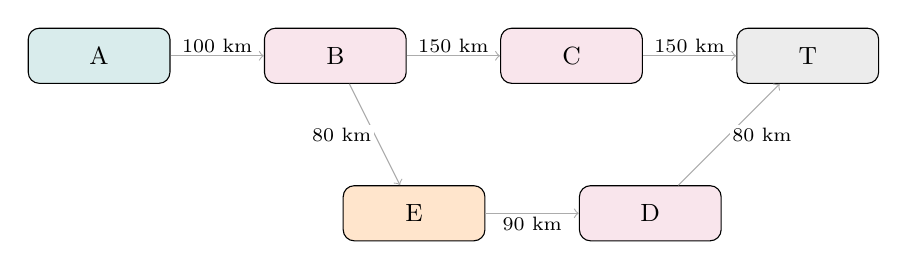
\begin{tikzpicture}[
    node/.style={draw, rounded corners=4pt, minimum width=1.8cm,
                 minimum height=0.7cm, font=\small, align=center},
    edge/.style={->, draw=gray!65},
    lbl/.style={font=\scriptsize, midway, fill=white, inner sep=1pt}
]

\node[node, fill=teal!15]   (A) at (0,0)   {A};
\node[node, fill=purple!10] (B) at (3,0)   {B};
\node[node, fill=purple!10] (C) at (6,0)   {C};
\node[node, fill=orange!20] (E) at (4,-2)  {E};
\node[node, fill=purple!10] (D) at (7,-2)  {D};
\node[node, fill=gray!15]   (T) at (9,0)   {T};

\draw[edge] (A) -- node[lbl,above]{100 km} (B);
\draw[edge] (B) -- node[lbl,above]{150 km} (C);
\draw[edge] (C) -- node[lbl,above]{150 km} (T);
\draw[edge] (B) -- node[lbl,left]{80 km}  (E);
\draw[edge] (E) -- node[lbl,below]{90 km} (D);
\draw[edge] (D) -- node[lbl,right]{80 km} (T);

\end{tikzpicture}
\caption{Running example network used in all worked examples.}
\label{fig:example_network}
\end{figure}

\begin{table}[ht]
\centering
\caption{Node roles and fuel prices in the running example.}
\label{tab:example_nodes}
\small
\begin{tabular}{@{}llll@{}}
\toprule
Node & Role & Fuel price (THB/L) & Initial status \\
\midrule
A & Origin station & 36 & Start with 28~L \\
B & Intermediate station & 44 & No initial fuel assignment \\
C & Intermediate station & 46 & No initial fuel assignment \\
E & Intermediate station & 24 & Global minimum price \\
D & Intermediate station & 38 & No initial fuel assignment \\
T & Destination & Not applicable & No fuel sold \\
\bottomrule
\end{tabular}
\end{table}

\begin{table}[ht]
\centering
\caption{Key path properties of the running example.}
\label{tab:example_paths}
\small
\begin{tabular}{@{}p{3.1cm}p{4.7cm}p{5.2cm}@{}}
\toprule
Path & Distance and fuel requirement & Cost implication \\
\midrule
$A\to B\to C\to T$ & 400~km, equivalent to 40~L & With $f_0=28$~L, at least 12~L must be purchased; the cheapest feasible purchase on this path is at~B, costing $12\times44=528$~THB \\
$A\to B\to E\to D\to T$ & 370~km, equivalent to 37~L & Arrival at~E occurs with 10~L remaining; purchasing only 9~L at 24~THB/L yields a total purchase cost of 216~THB \\
\bottomrule
\end{tabular}
\end{table}

The running example highlights the main challenge addressed in this study: the shortest path is not necessarily the least-cost path. Although the upper route is shorter in structure, the lower route is cheaper because it reaches the lowest-priced station before any large fuel purchase is required.

\section{Algorithmic Approaches}
\label{sec:algorithms}

\subsection{State-Expanded Dijkstra}
\label{subsec:dijkstra}

State-Expanded Dijkstra applies Dijkstra's shortest-path method to the state-expanded graph~$G^{*}$. Since each state encodes both location and remaining fuel, the algorithm jointly optimizes routing and refueling.

\begin{algorithm}[H]
\caption{State-Expanded Dijkstra}
\label{alg:dijkstra}
\begin{algorithmic}[1]
\Require $G^{*}$, source $s$, destination $t$, initial fuel $f_0$
\Ensure Minimum total fuel cost from $s$ to $t$
\State $\mathit{dist}[(v,f)] \gets \infty$ for all $(v,f)\in S$
\State $\mathit{dist}[(s,f_0)] \gets 0$
\State Min-heap $Q \gets \{(0, s, f_0)\}$
\While{$Q \neq \emptyset$}
    \State $(c,u,f) \gets \mathrm{EXTRACT\text{-}MIN}(Q)$
    \If{$u=t$}
        \State \Return $c$
    \EndIf
    \For{each travel edge $(u,v)$ with $f \ge d(u,v)/\eta$}
        \State Relax state $\bigl(v, f-d(u,v)/\eta\bigr)$ with cost $c$
    \EndFor
    \For{each purchase amount $b \in \{\varepsilon,\ldots,C-f\}$}
        \State Relax state $(u,f+b)$ with cost $c+b\,p(u)$
    \EndFor
\EndWhile
\State \Return $\min_f \mathit{dist}[(t,f)]$
\end{algorithmic}
\end{algorithm}

\begin{figure}[ht]
\centering
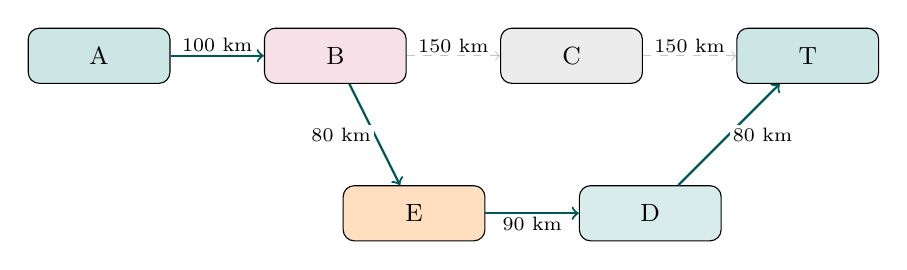
\begin{tikzpicture}[
    node/.style={draw, rounded corners=4pt, minimum width=1.8cm,
                 minimum height=0.7cm, font=\small, align=center},
    optedge/.style={->, thick, draw=teal!70!black},
    altedge/.style={->, dashed, draw=gray!45},
    lbl/.style={font=\scriptsize, midway, fill=white, inner sep=1pt}
]

\node[node, fill=teal!20]   (A) at (0,0)  {A};
\node[node, fill=purple!12] (B) at (3,0)  {B};
\node[node, fill=gray!15]   (C) at (6,0)  {C};
\node[node, fill=orange!25] (E) at (4,-2) {E};
\node[node, fill=teal!15]   (D) at (7,-2) {D};
\node[node, fill=teal!20]   (T) at (9,0)  {T};

\draw[optedge] (A) -- node[lbl,above]{100 km} (B);
\draw[optedge] (B) -- node[lbl,left]{80 km} (E);
\draw[optedge] (E) -- node[lbl,below]{90 km} (D);
\draw[optedge] (D) -- node[lbl,right]{80 km} (T);
\draw[altedge] (B) -- node[lbl,above]{150 km} (C);
\draw[altedge] (C) -- node[lbl,above]{150 km} (T);

\end{tikzpicture}
\caption{Optimal route identified by State-Expanded Dijkstra.}
\label{fig:dijkstra_route}
\end{figure}

\begin{table}[ht]
\centering
\caption{Decision trace for State-Expanded Dijkstra on the running example.}
\label{tab:dijkstra_trace}
\small
\begin{tabularx}{\textwidth}{c l c l X}
\toprule
Step & State $(v,f)$ & Cost & Interpretation & Notable successor states \\
\midrule
1 & $(A,28)$ & 0 & Initial state & $(B,18){:}0$ \\
2 & $(B,18)$ & 0 & Reach B without purchasing & $(E,10){:}0$, $(C,3){:}0$, refuel states at B \\
3 & $(E,10)$ & 0 & Reach low-price station E & $(E,19){:}216$, $(E,40){:}720$ \\
4 & $(C,3)$ & 0 & Reach C with insufficient fuel to finish & Additional refuel states at C \\
5 & $(E,19)$ & 216 & Purchase 9~L at E & $(D,11){:}216$ \\
6 & $(D,11)$ & 216 & Continue without further purchase & $(T,0){:}216$ \\
7 & $(T,0)$ & 216 & Goal reached & Return 216~THB \\
\bottomrule
\end{tabularx}
\end{table}

In this example, the algorithm correctly postpones refueling until station~E, where the fuel price is lowest. The resulting minimum cost is 216~THB.

\paragraph{Complexity.}
\[
T_{\mathrm{Dijkstra}}=O\!\left((EF+VF^{2})\log(VF)\right),
\qquad
\text{Space}=O(VF).
\]

\subsection{Greedy Baseline}
\label{subsec:greedy}

The greedy strategy uses a local rule: if a cheaper station is reachable in one hop, it purchases only enough fuel to reach that station; otherwise it fills the tank. This rule is computationally simple but not globally optimal.

\begin{algorithm}[H]
\caption{Greedy Fuel-Aware Routing}
\label{alg:greedy}
\begin{algorithmic}[1]
\Require Graph $G$, source $s$, destination $t$, initial fuel $f_0$, prices $p$
\Ensure Total fuel cost
\State $f \gets f_0$, $\mathit{cost} \gets 0$, $u \gets s$
\While{$u \neq t$}
    \State $R \gets \{v\in V : d(u,v)/\eta \le f \text{ and } p(v)<p(u)\}$
    \If{$R \neq \emptyset$}
        \State $v^{*} \gets \arg\min_{v\in R} d(u,v)$
        \State $b \gets \max\bigl(0, d(u,v^{*})/\eta - f\bigr)$
    \Else
        \State $b \gets C-f$
    \EndIf
    \State $\mathit{cost} \gets \mathit{cost} + b\,p(u)$
    \State $f \gets f+b$
    \State Travel to the next station and reduce $f$ accordingly
\EndWhile
\State \Return $\mathit{cost}$
\end{algorithmic}
\end{algorithm}

\begin{figure}[ht]
\centering
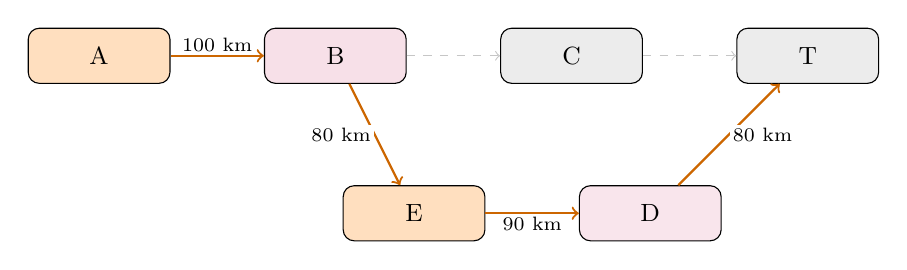
\begin{tikzpicture}[
    node/.style={draw, rounded corners=4pt, minimum width=1.8cm,
                 minimum height=0.7cm, font=\small, align=center},
    pathedge/.style={->, thick, draw=orange!80!black},
    altedge/.style={->, dashed, draw=gray!45},
    lbl/.style={font=\scriptsize, midway, fill=white, inner sep=1pt}
]

\node[node, fill=orange!25] (A) at (0,0)  {A};
\node[node, fill=purple!12] (B) at (3,0)  {B};
\node[node, fill=gray!15]   (C) at (6,0)  {C};
\node[node, fill=orange!25] (E) at (4,-2) {E};
\node[node, fill=purple!10] (D) at (7,-2) {D};
\node[node, fill=gray!15]   (T) at (9,0)  {T};

\draw[pathedge] (A) -- node[lbl,above]{100 km} (B);
\draw[pathedge] (B) -- node[lbl,left]{80 km} (E);
\draw[pathedge] (E) -- node[lbl,below]{90 km} (D);
\draw[pathedge] (D) -- node[lbl,right]{80 km} (T);
\draw[altedge] (B) -- (C);
\draw[altedge] (C) -- (T);

\end{tikzpicture}
\caption{Route obtained by the greedy baseline.}
\label{fig:greedy_route}
\end{figure}

\begin{table}[htbp]
\centering
\caption{Greedy decisions on the running example.}
\label{tab:greedy_trace}
\small
\begin{tabular}{@{}lllll@{}}
\toprule
Node & Arrival fuel & Decision & Fuel purchased & Running cost \\
\midrule
A & 28~L & No cheaper one-hop neighbour; fill tank & 12~L at 36~THB/L & 432~THB \\
B & 30~L & E is cheaper and reachable; buy nothing & 0~L & 432~THB \\
E & 22~L & No cheaper station reachable; fill tank & 18~L at 24~THB/L & 864~THB \\
D & 32~L & Continue to destination & 0~L & 864~THB \\
T & 22~L & Arrive & 0~L & 864~THB \\
\bottomrule
\end{tabular}
\end{table}

The greedy baseline performs poorly because it treats node~A in isolation. Although 28~L is already sufficient to reach node~E via node~B, the one-hop rule does not recognise this and triggers an unnecessary purchase at the origin. The total cost is 864~THB, which is four times the optimum.

\paragraph{Complexity.}
\[
T_{\mathrm{Greedy}}=O(V^{2}),
\qquad
\text{Space}=O(V).
\]

\subsection{Dynamic Programming Baseline}
\label{subsec:dp}

The DP baseline stores the minimum cost of reaching each node with each admissible fuel level. Formally, $\mathrm{DP}[v][f]$ denotes the minimum cost of arriving at node~$v$ with exactly $f$ litres remaining. In practice, the method evaluates all feasible purchase and travel combinations over the discretised state space.

\begin{algorithm}[H]
\caption{Dynamic Programming for Fuel-Aware Routing}
\label{alg:dp}
\begin{algorithmic}[1]
\Require Graph $G$, source $s$, destination $t$, prices $p$, capacity $C$
\Ensure Minimum total fuel cost
\State $\mathrm{DP}[v][f] \gets \infty$ for all $v\in V$ and $f\in F$
\State $\mathrm{DP}[s][f_0] \gets 0$
\For{each reachable state $(v,f)$ in the discretised state space}
    \For{each purchase amount $b\in\{0,\varepsilon,\ldots,C-f\}$}
        \State $f_{\mathrm{dep}} \gets f+b$
        \State $c_b \gets \mathrm{DP}[v][f] + b\,p(v)$
        \For{each neighbour $w$ with $f_{\mathrm{dep}}\ge d(v,w)/\eta$}
            \State $f_w \gets f_{\mathrm{dep}} - d(v,w)/\eta$
            \State $\mathrm{DP}[w][f_w] \gets \min\bigl(\mathrm{DP}[w][f_w], c_b\bigr)$
        \EndFor
    \EndFor
\EndFor
\State \Return $\min_f \mathrm{DP}[t][f]$
\end{algorithmic}
\end{algorithm}

\begin{figure}[ht]
\centering
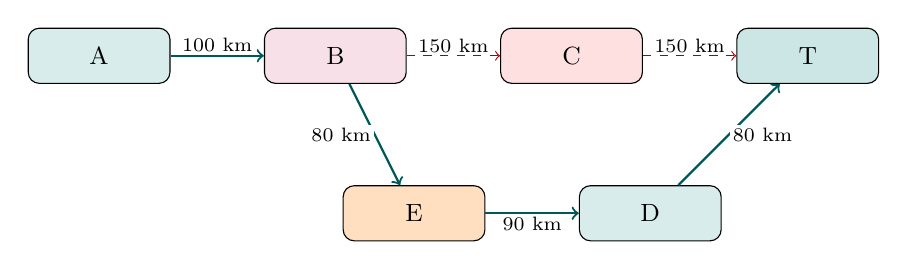
\begin{tikzpicture}[
    node/.style={draw, rounded corners=4pt, minimum width=1.8cm,
                 minimum height=0.7cm, font=\small, align=center},
    optedge/.style={->, thick, draw=teal!70!black},
    altedge/.style={->, dashed, draw=red!65!black},
    lbl/.style={font=\scriptsize, midway, fill=white, inner sep=1pt}
]

\node[node, fill=teal!15]   (A) at (0,0)  {A};
\node[node, fill=purple!12] (B) at (3,0)  {B};
\node[node, fill=red!12]    (C) at (6,0)  {C};
\node[node, fill=orange!25] (E) at (4,-2) {E};
\node[node, fill=teal!15]   (D) at (7,-2) {D};
\node[node, fill=teal!20]   (T) at (9,0)  {T};

\draw[optedge] (A) -- node[lbl,above]{100 km} (B);
\draw[optedge] (B) -- node[lbl,left]{80 km} (E);
\draw[optedge] (E) -- node[lbl,below]{90 km} (D);
\draw[optedge] (D) -- node[lbl,right]{80 km} (T);
\draw[altedge] (B) -- node[lbl,above]{150 km} (C);
\draw[altedge] (C) -- node[lbl,above]{150 km} (T);

\end{tikzpicture}
\caption{Optimal and suboptimal branches evaluated by Dynamic Programming.}
\label{fig:dp_route}
\end{figure}

% In the preamble, if not already added:
% \usepackage{tabularx}
% \usepackage{array}

\begin{table}[htbp]
\centering
\caption{Selected dynamic programming states for the running example.}
\label{tab:dp_trace}
\small
\setlength{\tabcolsep}{5pt}
\renewcommand{\arraystretch}{1.15}
\begin{tabularx}{\linewidth}{@{}
>{\raggedright\arraybackslash}p{2.8cm}
>{\raggedright\arraybackslash}X
>{\raggedright\arraybackslash}p{2.5cm}
>{\raggedright\arraybackslash}X
>{\raggedleft\arraybackslash}p{1.4cm}
@{}}
\toprule
State & Interpretation & Purchase & Successor state & Cost \\
\midrule
$\mathrm{DP}[A][28]=0$ & Initial state & 0\,L & $\mathrm{DP}[B][18]=0$ & 0 \\
$\mathrm{DP}[B][18]=0$ & Reach B without purchase & 0\,L & $\mathrm{DP}[E][10]=0$ & 0 \\
$\mathrm{DP}[E][10]=0$ & Reach E at the minimum-price station & 9\,L at 24\,THB/L & $\mathrm{DP}[D][11]=216$ & 216 \\
$\mathrm{DP}[C][3]=0$ & Alternative route through C & 12\,L at 46\,THB/L & $\mathrm{DP}[T][0]=552$ via C & 552 \\
$\mathrm{DP}[T][0]$ & Best final value retained & -- & Optimal solution & 216 \\
\bottomrule
\end{tabularx}
\end{table}

The DP baseline evaluates both the optimal branch through~E and the more expensive branch through~C, retaining the minimum value for each state. For the running example, the optimal total remains 216~THB.

\paragraph{Complexity.}
\[
T_{\mathrm{DP}}=
\begin{cases}
O(VF^{2}\Delta), & \text{naive implementation},\\
O(EF), & \text{optimized implementation},
\end{cases}
\qquad
\text{Space}=O(VF),
\]
where $\Delta$ denotes the maximum out-degree.

\subsection{Standard A* Search}
\label{subsec:astar}

Standard A* augments the state-expanded search with a lower-bound estimate of the remaining travel cost. The heuristic is defined as
\[
h(v)=\frac{d_{\mathrm{geo}}(v,t)}{\eta}\,p_{\min},
\]
where $d_{\mathrm{geo}}(v,t)$ is the straight-line distance from node~$v$ to the destination and $p_{\min}$ is the global minimum fuel price in the network. This heuristic is admissible because it assumes that all remaining fuel can be purchased at the lowest possible price.

\begin{algorithm}[H]
\caption{A* Search for Fuel-Aware Routing}
\label{alg:astar}
\begin{algorithmic}[1]
\Require $G^{*}$, source $s$, destination $t$, heuristic $h$, initial fuel $f_0$
\Ensure Minimum total fuel cost from $s$ to $t$
\State $g[(v,f)] \gets \infty$ for all $(v,f)\in S$
\State $g[(s,f_0)] \gets 0$
\State Min-heap $Q \gets \{(h(s), s, f_0)\}$
\While{$Q \neq \emptyset$}
    \State $(\_,u,f) \gets \mathrm{EXTRACT\text{-}MIN}(Q)$
    \If{$u=t$}
        \State \Return $g[(t,f)]$
    \EndIf
    \For{each travel edge $(u,v)$ with $f \ge d(u,v)/\eta$}
        \State $g' \gets g[(u,f)]$
        \State $f' \gets f-d(u,v)/\eta$
        \If{$g' < g[(v,f')]$}
            \State $g[(v,f')] \gets g'$
            \State Push $\bigl(g'+h(v), v, f'\bigr)$ to $Q$
        \EndIf
    \EndFor
    \For{each purchase amount $b\in\{\varepsilon,\ldots,C-f\}$}
        \State $g' \gets g[(u,f)] + b\,p(u)$
        \State $f' \gets f+b$
        \If{$g' < g[(u,f')]$}
            \State $g[(u,f')] \gets g'$
            \State Push $\bigl(g'+h(u), u, f'\bigr)$ to $Q$
        \EndIf
    \EndFor
\EndWhile
\end{algorithmic}
\end{algorithm}

\begin{figure}[ht]
\centering
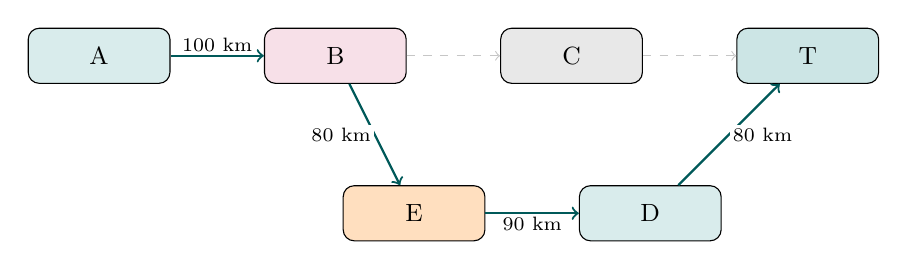
\begin{tikzpicture}[
    node/.style={draw, rounded corners=4pt, minimum width=1.8cm,
                 minimum height=0.7cm, font=\small, align=center},
    optedge/.style={->, thick, draw=teal!70!black},
    altedge/.style={->, dashed, draw=gray!45},
    lbl/.style={font=\scriptsize, midway, fill=white, inner sep=1pt}
]

\node[node, fill=teal!15]   (A) at (0,0)  {A};
\node[node, fill=purple!12] (B) at (3,0)  {B};
\node[node, fill=gray!18]   (C) at (6,0)  {C};
\node[node, fill=orange!25] (E) at (4,-2) {E};
\node[node, fill=teal!15]   (D) at (7,-2) {D};
\node[node, fill=teal!20]   (T) at (9,0)  {T};

\draw[optedge] (A) -- node[lbl,above]{100 km} (B);
\draw[optedge] (B) -- node[lbl,left]{80 km} (E);
\draw[optedge] (E) -- node[lbl,below]{90 km} (D);
\draw[optedge] (D) -- node[lbl,right]{80 km} (T);
\draw[altedge] (B) -- (C);
\draw[altedge] (C) -- (T);

\end{tikzpicture}
\caption{Optimal route identified by Standard A*.}
\label{fig:astar_route}
\end{figure}

\begin{table}[ht]
\centering
\caption{Illustrative A* expansion priorities on the running example.}
\label{tab:astar_trace}
\small
\begin{tabular}{@{}lllll@{}}
\toprule
State & $g$ & $h(v)$ & $f$-score & Interpretation \\
\midrule
$(A,28)$ & 0 & 912 & 912 & Initial state \\
$(B,18)$ & 0 & 672 & 672 & Expanded after travel from A \\
$(E,10)$ & 0 & 504 & 504 & Preferred low-cost branch \\
$(C,3)$ & 0 & 360 & 360 & Reachable, but insufficient fuel to finish \\
$(E,19)$ & 216 & 504 & 720 & Purchase 9~L at E \\
$(D,11)$ & 216 & 264 & 480 & Continue toward destination \\
$(T,0)$ & 216 & 0 & 216 & Goal state returned \\
\bottomrule
\end{tabular}
\end{table}

Standard A* still returns the optimal cost of 216~THB. However, because the heuristic depends only on node position and not on fuel level, some less useful states remain competitive in the priority queue.

\paragraph{Complexity.}
\[
T_{\mathrm{A^{*}}}=O\!\left((EF+VF^{2})\log(VF)\right)
\quad \text{in the worst case},
\qquad
\text{Space}=O(VF).
\]

\subsection{Refuel A* (RF-A*)}
\label{subsec:rfastar}

RF-A* is a refueling-oriented variant of A* that applies a fuel-agnostic lower bound,
\[
h_{\mathrm{RF}}(v)=\frac{d_{\mathrm{geo}}(v,t)}{\eta}\,p_{\min}.
\]
Although it encourages movement toward the destination, it does not distinguish between states with different fuel levels at the same node.

\begin{algorithm}[H]
\caption{RF-A* Search for Fuel-Aware Routing}
\label{alg:rfastar}
\begin{algorithmic}[1]
\Require $G^{*}$, source $s$, destination $t$, initial fuel $f_0$
\Ensure Minimum total fuel cost from $s$ to $t$
\State $u \gets s$, $f \gets f_0$, $\mathit{totalCost} \gets 0$
\While{$u \neq t$}
    \State Select the next target as a cheaper reachable station, or $t$ if none exists
    \State Run A* from $(u,f)$ to the selected target using $h_{\mathrm{RF}}$
    \State Append the segment cost and update the current state
    \If{$u \neq t$}
        \State Refuel according to the chosen segment decision
    \EndIf
\EndWhile
\State \Return $\mathit{totalCost}$
\end{algorithmic}
\end{algorithm}

\begin{figure}[ht]
\centering
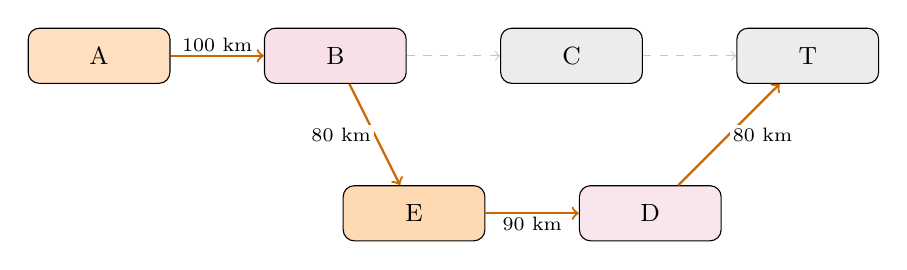
\begin{tikzpicture}[
    node/.style={draw, rounded corners=4pt, minimum width=1.8cm,
                 minimum height=0.7cm, font=\small, align=center},
    pathedge/.style={->, thick, draw=orange!80!black},
    altedge/.style={->, dashed, draw=gray!45},
    lbl/.style={font=\scriptsize, midway, fill=white, inner sep=1pt}
]

\node[node, fill=orange!25] (A) at (0,0)  {A};
\node[node, fill=purple!12] (B) at (3,0)  {B};
\node[node, fill=gray!15]   (C) at (6,0)  {C};
\node[node, fill=orange!30] (E) at (4,-2) {E};
\node[node, fill=purple!10] (D) at (7,-2) {D};
\node[node, fill=gray!15]   (T) at (9,0)  {T};

\draw[pathedge] (A) -- node[lbl,above]{100 km} (B);
\draw[pathedge] (B) -- node[lbl,left]{80 km} (E);
\draw[pathedge] (E) -- node[lbl,below]{90 km} (D);
\draw[pathedge] (D) -- node[lbl,right]{80 km} (T);
\draw[altedge] (B) -- (C);
\draw[altedge] (C) -- (T);

\end{tikzpicture}
\caption{Route obtained by RF-A* on the running example.}
\label{fig:rfastar_route}
\end{figure}

\begin{table}[ht]
\centering
\caption{RF-A* decisions on the running example.}
\label{tab:rfastar_trace}
\small
\begin{tabular}{@{}lllll@{}}
\toprule
Node & $h_{\mathrm{RF}}(v)$ & Arrival fuel & Decision & Running cost \\
\midrule
A & 912 & 28~L & Fill 12~L at 36~THB/L & 432~THB \\
B & 672 & 30~L & Buy nothing & 432~THB \\
E & 504 & 22~L & Fill 18~L at 24~THB/L & 864~THB \\
D & 264 & 32~L & Continue & 864~THB \\
T & 0 & 22~L & Arrive & 864~THB \\
\bottomrule
\end{tabular}
\end{table}

RF-A* follows the same route as the optimal solution but makes poor refueling decisions. Because $h_{\mathrm{RF}}(v)$ is independent of fuel level, states $(A,28)$ and $(A,40)$ receive the same heuristic treatment, causing the algorithm to over-purchase at the origin. The total cost is therefore 864~THB.

\paragraph{Complexity.}
\[
T_{\mathrm{RF\text{-}A^{*}}}=O\!\left((EF+VF^{2})\log(VF)\right),
\qquad
\text{Space}=O(VF).
\]

\subsection{Partial-Fill A* (PF-A*)}
\label{subsec:pfastar}

PF-A* is the proposed extension. It replaces the fuel-agnostic lower bound with a fuel-level-aware heuristic,
\[
h_{\mathrm{PF}}(v,f)=\max\!\left(\frac{d_{\mathrm{geo}}(v,t)}{\eta}-f,\,0\right)\,p_{\min}^{\mathrm{reach}}(v,f),
\]
where $p_{\min}^{\mathrm{reach}}(v,f)$ denotes the minimum fuel price among stations reachable from~$v$ given the current fuel state~$f$. The heuristic estimates the amount of additional fuel still required and weights it by the cheapest reachable purchase price. This yields a tighter lower bound than RF-A*.

\begin{algorithm}[H]
\caption{PF-A* Search for Fuel-Aware Routing}
\label{alg:pfastar}
\begin{algorithmic}[1]
\Require $G^{*}$, source $s$, destination $t$, initial fuel $f_0$
\Ensure Minimum total fuel cost from $s$ to $t$
\State Precompute $p_{\min}^{\mathrm{reach}}(v,f)$ for all feasible states
\State $g[(v,f)] \gets \infty$ for all $(v,f)\in S$
\State $g[(s,f_0)] \gets 0$
\State Min-heap $Q \gets \{(h_{\mathrm{PF}}(s,f_0), s, f_0)\}$
\While{$Q \neq \emptyset$}
    \State $(\_,u,f) \gets \mathrm{EXTRACT\text{-}MIN}(Q)$
    \If{$u=t$}
        \State \Return $g[(t,f)]$
    \EndIf
    \For{each travel edge $(u,v)$ with $f \ge d(u,v)/\eta$}
        \State $g' \gets g[(u,f)]$
        \State $f' \gets f-d(u,v)/\eta$
        \If{$g' < g[(v,f')]$}
            \State $g[(v,f')] \gets g'$
            \State Push $\bigl(g'+h_{\mathrm{PF}}(v,f'), v, f'\bigr)$ to $Q$
        \EndIf
    \EndFor
    \For{each purchase amount $b\in\{\varepsilon,\ldots,C-f\}$}
        \State $g' \gets g[(u,f)] + b\,p(u)$
        \State $f' \gets f+b$
        \If{$g' < g[(u,f')]$}
            \State $g[(u,f')] \gets g'$
            \State Push $\bigl(g'+h_{\mathrm{PF}}(u,f'), u, f'\bigr)$ to $Q$
        \EndIf
    \EndFor
\EndWhile
\end{algorithmic}
\end{algorithm}

For the initial state $(A,28)$ in the running example,
\begin{itemize}
    \item $d_{\mathrm{geo}}(A,T)/\eta = 380/10 = 38$~L,
    \item the additional fuel lower bound is $\max(38-28,0)=10$~L,
    \item the cheapest price reachable from $(A,28)$ is 36~THB/L at node~A, because node~E is not directly reachable from A in a single hop,
    \item therefore $h_{\mathrm{PF}}(A,28)=10\times36=360$.
\end{itemize}
This value is substantially tighter than the RF-A* estimate of $38\times24=912$, and it preserves the distinction between partially fuelled and fully fuelled states at the same node.

\begin{figure}[ht]
\centering
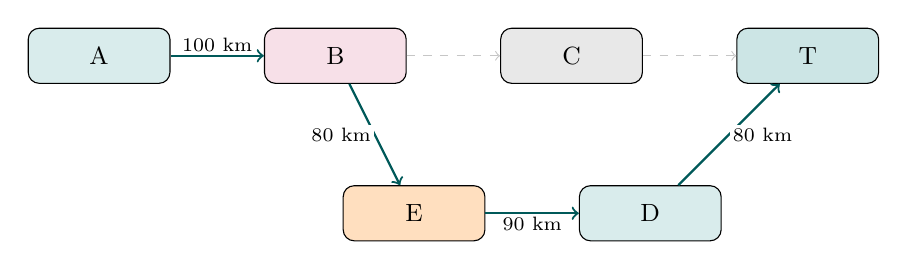
\begin{tikzpicture}[
    node/.style={draw, rounded corners=4pt, minimum width=1.8cm,
                 minimum height=0.7cm, font=\small, align=center},
    optedge/.style={->, thick, draw=teal!70!black},
    altedge/.style={->, dashed, draw=gray!45},
    lbl/.style={font=\scriptsize, midway, fill=white, inner sep=1pt}
]

\node[node, fill=teal!15]   (A) at (0,0)  {A};
\node[node, fill=purple!12] (B) at (3,0)  {B};
\node[node, fill=gray!18]   (C) at (6,0)  {C};
\node[node, fill=orange!25] (E) at (4,-2) {E};
\node[node, fill=teal!15]   (D) at (7,-2) {D};
\node[node, fill=teal!20]   (T) at (9,0)  {T};

\draw[optedge] (A) -- node[lbl,above]{100 km} (B);
\draw[optedge] (B) -- node[lbl,left]{80 km} (E);
\draw[optedge] (E) -- node[lbl,below]{90 km} (D);
\draw[optedge] (D) -- node[lbl,right]{80 km} (T);
\draw[altedge] (B) -- (C);
\draw[altedge] (C) -- (T);

\end{tikzpicture}
\caption{Optimal route identified by PF-A*.}
\label{fig:pfastar_route}
\end{figure}

\begin{table}[ht]
\centering
\caption{PF-A* decisions on the running example.}
\label{tab:pfastar_trace}
\small
\begin{tabular}{@{}lllll@{}}
\toprule
State & Heuristic value & Action & Purchase cost & Running cost \\
\midrule
$(A,28)$ & $\max(38-28,0)\times36 = 360$ & Do not purchase & 0 & 0 \\
$(B,18)$ & $\max(28-18,0)\times24 = 240$ & Do not purchase & 0 & 0 \\
$(E,10)$ & $\max(21-10,0)\times24 = 264$ & Purchase 9~L at E & 216~THB & 216~THB \\
$(D,11)$ & $\max(11-11,0)\times24 = 0$ & Continue & 0 & 216~THB \\
$(T,0)$ & 0 & Arrive & 0 & 216~THB \\
\bottomrule
\end{tabular}
\end{table}

PF-A* achieves the optimal solution while avoiding the unnecessary origin purchase made by Greedy and RF-A*. Its practical advantage is not a better worst-case asymptotic bound, but a more informative ordering of states during search.

\paragraph{Complexity.}
\[
T_{\mathrm{PF\text{-}A^{*}}}=O\!\left((EF+VF^{2})\log(VF)\right),
\qquad
\text{Space}=O(VF).
\]

\section{Effect of Variable Purchase Decisions}
\label{sec:variable_purchase}

A central issue in this research is the effect of allowing partial refueling decisions.

\paragraph{Full-tank-only model.}
If the driver must always fill the tank completely, fuel level no longer behaves as a decision variable. The problem reduces to route selection over the original graph, with each refueling event fixed at capacity. This model is computationally simpler but may purchase more fuel than necessary.

\paragraph{Variable-purchase model.}
If the driver may buy any amount in the interval $[0,C-f]$, fuel level becomes part of the decision process. The algorithm must therefore track both node and remaining fuel, leading to the state-expanded model with state complexity $O(VF)$.

For the running example, the best full-tank-style decision costs 528~THB, whereas the best variable-purchase decision costs 216~THB. This represents a 59\% reduction in purchase cost.


\begin{table}[htbp]
\centering
\caption{Comparison of modelling assumptions, state-space size, and representative solution methods.}
\label{tab:model_comparison}
\small
\setlength{\tabcolsep}{5pt}
\renewcommand{\arraystretch}{1.15}
\begin{tabularx}{\linewidth}{@{}
>{\raggedright\arraybackslash}p{2.5cm}
>{\raggedright\arraybackslash}p{2.9cm}
>{\centering\arraybackslash}p{1.7cm}
>{\raggedright\arraybackslash}X
>{\centering\arraybackslash}p{1.6cm}
@{}}
\toprule
Model & Representative algorithm & State space & Time complexity & Optimality \\
\midrule
Full-tank-only & Dijkstra on $G$ & $O(V)$ & $O(E\log V)$ & No \\
Full-tank-only & Greedy fill policy & $O(V)$ & $O(V^{2})$ & No \\
Variable purchase & Dijkstra on $G^{*}$ & $O(VF)$ & $O((EF + VF^{2})\log(VF))$ & Yes \\
Variable purchase & DP & $O(VF)$ & $O(EF)$ in optimized form & Yes \\
Variable purchase & PF-A* & $O(VF)$ & $O((EF + VF^{2})\log(VF))$ & Yes \\
\bottomrule
\end{tabularx}
\end{table}

\section{Dataset Description}

\subsection{Real-World Data}

The real-world experiments use road-network and station-location data derived from OpenStreetMap point-of-interest information for Thailand, with fuel stations identified through the \texttt{amenity=fuel} tag. The drivable road graph is extracted with OSMnx, and road distances between stations are computed over the road network rather than by straight-line approximation.

Fuel-price information is collected from Thai retail fuel-price sources and aligned to station locations by fuel grade and region. Where necessary, fallback price records are used to maintain experimental completeness.

Three representative travel corridors are considered:
\begin{itemize}
    \item Bangkok to Chiang Mai, representing a long northern corridor,
    \item Bangkok to Phuket, representing a long southern corridor,
    \item Bangkok to Khon Kaen, representing a medium-length northeastern corridor.
\end{itemize}

\subsection{Synthetic Data Generation}

Synthetic networks are generated to evaluate algorithm behavior under controlled changes in station density, graph size, fuel capacity, initial fuel, and price variance. The procedure is as follows:
\begin{enumerate}
    \item Generate $N$ station locations uniformly within a bounded region.
    \item Connect stations whose separation is within the maximum travel range $\eta C$.
    \item Assign edge distances from scaled Euclidean separations.
    \item Sample fuel prices from a bounded distribution with controllable variance.
    \item Select origin--destination pairs subject to a minimum separation requirement.
    \item Construct both the base graph~$G$ and the state-expanded graph~$G^{*}$.
\end{enumerate}

\begin{table}[htbp]
\centering
\caption{Synthetic data generation parameters.}
\label{tab:synth_params}
\small
\setlength{\tabcolsep}{5pt}
\renewcommand{\arraystretch}{1.15}
\begin{tabularx}{\linewidth}{@{}
>{\raggedright\arraybackslash}p{3.3cm}
>{\raggedright\arraybackslash}p{2.7cm}
>{\raggedright\arraybackslash}X
>{\raggedright\arraybackslash}p{3.2cm}
@{}}
\toprule
Parameter & Range & Purpose & Relevance \\
\midrule
Station density & 0.1--5 per 100\,km & Sparse to dense networks & All models \\
Price variance & 0--20\% & Low to high price dispersion & All models \\
Tank capacity $C$ & 20, 40, 60, 80\,L & Severity of fuel-range constraint & All models \\
Initial fuel $f_0$ & $0.25C$ to $1.0C$ & Partially filled and nearly full starts & Variable-purchase models \\
Origin--destination distance & 100--1000\,km & Short to long journeys & All models \\
Graph size $|V|$ & 100, 1000, 10000 & Scalability analysis & All models \\
Purchase model & Full-tank or variable & Model comparison & Comparative experiments \\
\bottomrule
\end{tabularx}
\end{table}

In summary, this chapter defines the mathematical model, presents the baseline and proposed algorithms, and establishes the datasets used for evaluation. The proposed PF-A* method differs from the baselines primarily through its fuel-level-aware heuristic, which is designed to improve search guidance without sacrificing optimality.
